\documentclass[7pt]{article}
\usepackage{amsmath}
\usepackage{graphicx}
\usepackage{caption}
\usepackage[landscape]{geometry}
\usepackage{multicol}
\usepackage{enumitem}
\usepackage{amssymb}
\usepackage{float}
\usepackage{geometry}
 \geometry{
 a4paper,
 total={285mm,185mm},
 left=10mm,
 top=10mm,
 }

\setcounter{section}{7}
\setlength\columnseprule{0.5pt}
\setlength{\parindent}{0pt}
\graphicspath{ {images/} }

\begin{document}
\begin{multicols*}{3}
	
\section{Elektromagnetismus}

\subsection{Coulombsche Gesetz}

Die \textbf{Coulombsche (elektrostatische) Kraft}, die eine Punktladung $Q$ (Quelle) auf eine Ladung $q$ (Testladung) aus{\"u}bt, ist gleich:

\begin{equation*}
	F = \frac{1}{4\pi\varepsilon_0}\frac{qQ}{r^2} \quad [N]
\end{equation*}

wobei $\varepsilon_0$ die elektrische Feldkonstante und $r$ der Ortsvektor der Ladung $q$ ist. Der Ursprung des Koordinatensystems ist der Mittelpunkt der Ladung $Q$. \\

\subsection{Elektrisches Feld}

Das \textbf{elektrische Feld} ist definiert als:
\begin{equation*}
	E(r) \equiv \frac{F(r)}{q} = \frac{1}{4\pi\varepsilon_0}\frac{Q}{r^2}
\end{equation*}

Das zweite Teilchen der Ladung $q$ und Masse $m$ sp{\"u}rt die Kraft des Feldes:
\begin{equation*}
	F(r) = qE(r)
\end{equation*}

F{\"u}r eine positive Ladung $q$ zeit die Kraft in die Richtung des Feldes. \\

Es erf{\"a}hrt eine \textbf{Beschleunigung}:
\begin{equation*}
	a = \frac{q}{m}E
\end{equation*}

\subsubsection{Elektrische Feldlinien}

\begin{enumerate}
	\item Beginnen bei positiven Ladungen und enden bei negativen Ladungen oder im Unendlichen
	\item An bestimmten Punkt ist die \textbf{Liniendichte} proportional zur St{\"a}rke des Feldes an diesem Punkt
	\item Um einzelne Punktladungen sind die Linien kugelsymmetrisch verteilt
	\item Anzahl Feldlinien um eine Punktladung ist zur Gr{\"o}sse der Ladung proportional
\end{enumerate}

\subsection{Magnetisches Feld}

\begin{description}[labelindent=16pt,style=multiline,leftmargin=2.5cm, noitemsep]
	\item[Richtung:] Elektrische Feldlinien beginnen bei positiven Ladungen und enden bei negativen.\newline
		Magnetische Feldlinien bilden geschlossene Schleifen Richtung S{\"u}dpol.
	\item[Kraft:] Das elektrische Feld {\"u}bt seine Kraft l{\"a}ngs der Feldlinien aus. \newline
				 Die Kraft des magnetischen Feldes wirkt nur auf bewegte Ladungen und zwar senkrecht zum B-Feld und zur Bewegungsrichtung.
\end{description}

\begin{center}
	\begin{center}
		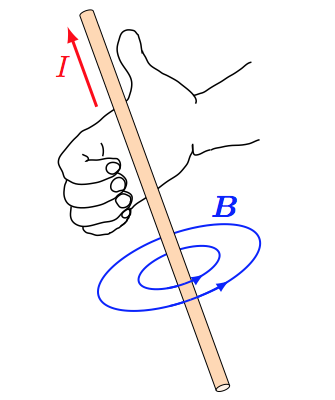
\includegraphics[width=80pt]{images/mf/draht}
		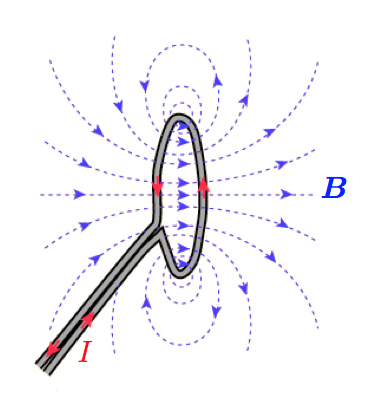
\includegraphics[width=80pt]{images/mf/ring}
	\end{center}
	\begin{center}
		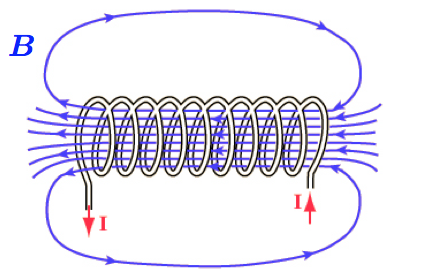
\includegraphics[width=80pt]{images/mf/solenoid}
		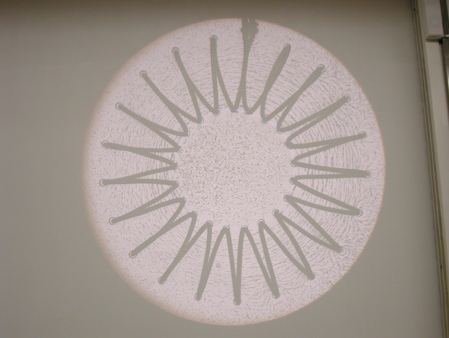
\includegraphics[width=80pt]{images/mf/torus}
	\end{center}
Magnetisches Feld durch einen Draht, Ring, Solenoid, Torus
\end{center}

\subsection{Energie im elektrischen Feld}

Es wird \textbf{Arbeit} geleistet, wenn der Abstand zwischen zwei ungleichnamigen (ziehen sich an) Ladungen vergr{\"o}ssert wird bzw. erh{\"a}lt man Arbeit, wenn die Ladungen gleichnamig sind. Diese Arbeit wird als \textbf{elektrische potentielle Energie} gespeichert.

\begin{equation*}
	E^e_{pot}(r) = \frac{1}{4\pi\varepsilon_0}\frac{q_1q_2}{r}
\end{equation*}

\subsubsection{Elektrisches Potential}

Das \textbf{elektrische Potential} $V$ ist ein Skalarfeld und entspricht der potentiellen Energie f{\"u}r eine Einheitsladung:
\begin{equation*}
	V(r) = \frac{E^e_{pot}(r)}{q} \quad [V(r)] = V
\end{equation*}

\subsubsection{Elektrische Spannung}

Die \textbf{elektrische Spannung} ist gleich dem Potentialunterschied zwischen zwei Punkten:
\begin{equation*}
	U_{1,2} = V(r_1)-V(r_2) = \int_{r_1}^{r_2}E\ dr \quad [U] = V
\end{equation*}

\subsection{Elektrische Ladung in elektrischen und magnetischen Feldern}

\subsubsection{Lorentzkraft}

Die \textbf{allgemeine elektromagnetische Kraft} ist gleich
\begin{equation*}
	F = F_E + F_B = q(E + v\times B)
\end{equation*}
wobei $E$ das elektrische Feld un $B$ das magnetische Feld ist. Sie haben die Einheiten:

\begin{equation*}
	[E] = \frac{N}{C},\quad [B] = \frac{N}{C\cdot \frac{m}{s}} = T
\end{equation*}

\paragraph{Magnetische Kraft:}
\begin{enumerate}
	\item Proportional zur Geschwindigkeit. Wirkt nur auf bewegte Teilchen.
	\item Wirkt senkrecht zur Bewegungsrichtung und zur Richtung des Feldes
	\item $|F_B| = |q||v||B|\sin(\alpha)$, wobei $\alpha$ der Winkel zwischen $v$ und $B$ ist
\end{enumerate}

\subsection{Elektrische Strom}

\subsubsection{Stromst{\"a}rke}

Die \textbf{elektrische Stromst{\"a}rke} ist definiert als:
\begin{equation*}
	I(t) = \frac{\Delta Q}{\Delta t} = -enAv_D \quad [I] = A = \frac{C}{s}
\end{equation*}
wobei $v_D$ der Driftgeschwindigkeit und $n$ der Dichte der beweglichen Elektronen entspricht. \\

\emph{Die positive Stromrichtung folgt der Flussrichtung der positiven Ladungen.} \\

\paragraph{Driftgeschwindigkeit:} \mbox{} \\

Gegeben:
\begin{description}[labelindent=16pt,style=multiline,leftmargin=4cm, noitemsep]
	\item[Kupferdraht:] ein Elektron pro Atom, $8.93 \frac{g}{cm^3}$, $63.5 \frac{g}{mol}$
	\item[Querschnittsfl{\"a}che:] $1mm^2$
	\item[Stromst{\"a}rke:] $1 A$
\end{description}

\begin{equation*}
\begin{split}
	n & = \frac{8.93 \frac{g}{cm^3} \cdot \frac{6 \cdot 10^{23}}{mol}}{63.5 \frac{g}{mol}} = 8.5 \cdot 10^{22} \frac{\text{Elektronen}}{cm^3} \\
	|v_D| & = \frac{I}{enA} = 0.07 \frac{mm}{s}
\end{split}
\end{equation*}

Die Driftgeschwindigkeit l{\"a}sst sich auch mit der Beschleunigung $a$ und der mittleren Zeit zwischen zwei Elektron-Ion Kollisionen $\tau$ absch{\"a}tzen:
\begin{equation*}
	v_D = a\tau = \frac{-eE}{m}\tau = -\mu E
\end{equation*}

\subsubsection{Ohmsches Gesetz}

\begin{equation*}
	U_{AB} = RI = (\frac{L}{\sigma A})I \quad [\sigma] = \frac{A}{Vm} = (\Omega m)^{-1}
\end{equation*}

wobei $\sigma$ die \textbf{Leitf{\"a}higkeit} und $L$ die L{\"a}nge des Leiters ist.

\subsection{Kraft auf elektrischen Strom}

Die Gesamtkraft auf einen Leiter der Querschnittsfl{\"a}che $A$ und L{\"a}nge $L$ ist:
\begin{equation*}
	F = ALn(-e)v_D \times B = L(-enAv_D)\times B = LI \times B
\end{equation*}

F{\"u}r ein differentielles Element des Stroms ist sie gleich:
\begin{equation*}
	dF = L\ dI \times B = I\ dL\times B
\end{equation*}

\subsubsection{Kraft zwischen zwei parallelen Leitern}

\begin{center}
	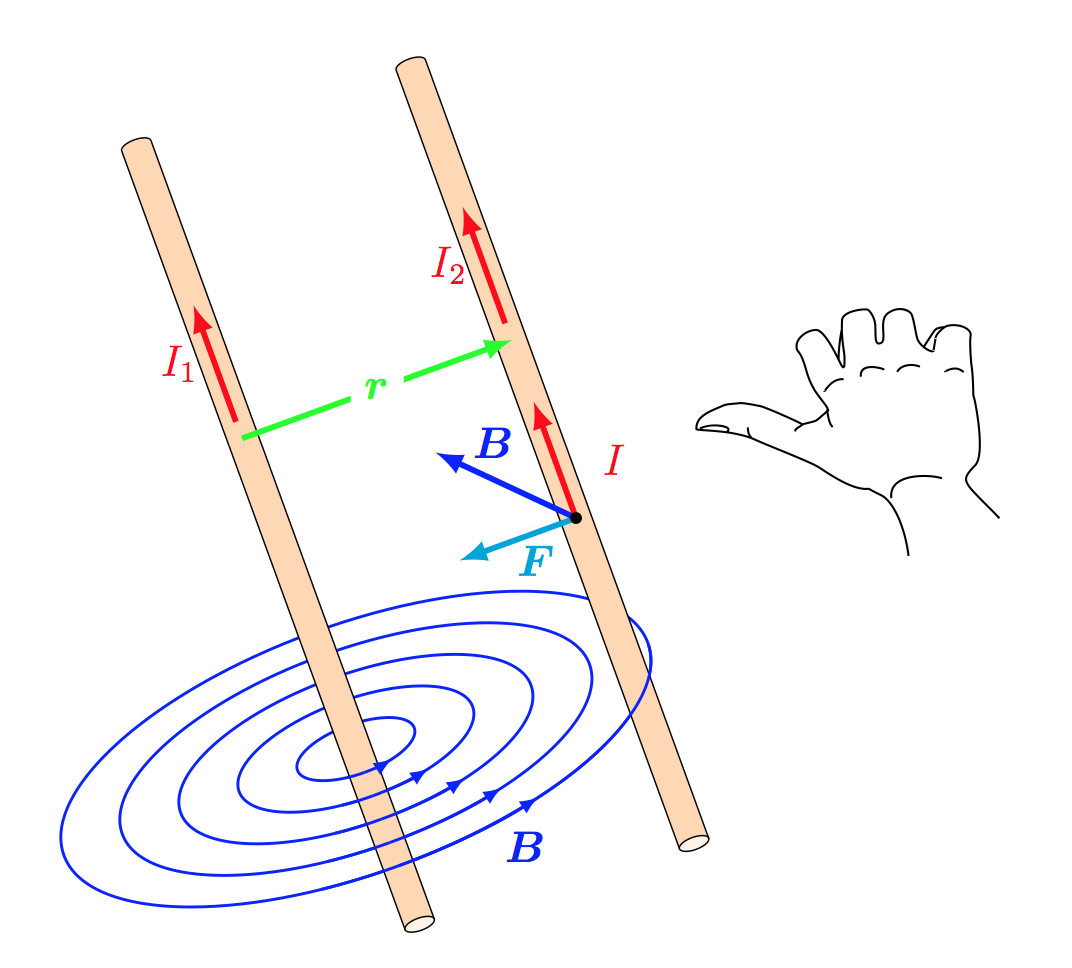
\includegraphics[width=150pt]{images/parallele_leiter}
\end{center}

\begin{equation*}
	F = LI \times B
\end{equation*}

Fliessen die zwei Str{\"o}me in die gleiche Richtung, so ziehen sich die Leiter an.

\subsection{Elektrische Kapazit{\"a}t}

In einem \textbf{Kondensator} wird Energie in einem elektrischen Feld gespeichert.

Die \textbf{Kapazit{\"a}t des Kondensators} $C$ ist gleich:
\begin{equation*}
	C = \frac{Q}{V} \quad [C] = F = \frac{C}{V}
\end{equation*}

wobei $Q$ die Ladung des Kondensators und $V$ die Potenzialdifferenz zwischen den Platten ist. \\

Die \textbf{gespeicherte Energie} (bzw. geleistete Arbeit zum Laden) ist gleich:
\begin{equation*}
	E = \frac{Q^2}{2C} = \frac{1}{2}CV^2
\end{equation*}

\subsection{Ladungs- und Stromdichte}

\subsection{Ladungsdichte}

Die \textbf{Raumladungsdichte} ist ein Skalarfeld und ist gleich:

\begin{equation*}
	\rho(r) = \frac{dq}{dV}
\end{equation*}

\subsubsection{Stromdichte}

Die \textbf{Stromdichte} bezeichnet Stromst{\"a}rke pro Fl{\"a}che und ist gleich:
\begin{equation*}
	j = \frac{I}{A}
\end{equation*}

\textbf{Vektoriel} ist sie gleich:
\begin{equation*}
	I = \iint_A j(r)\ dA
\end{equation*}

\subsubsection{Kontinuit{\"a}tsgleichung}

Sie besagt, dass wenn sich die elektrische Ladung in einem Punkt $r$ {\"a}ndert, muss in diesem Punkt ein elektrischer Strom fliessen.

\begin{equation*}
	\frac{\partial\rho(r)}{\partial t} + \nabla\cdot j(r) = 0
\end{equation*}

\subsection{Elektrischer Fluss}

Der elektrische Fluss durch eine Fl{\"a}che $A$ wird definiert als der Fluss des elektrischen Feldes durch die Fl{\"a}che:

\begin{equation*}
	\Phi_E = \iint_A E\ dA
\end{equation*}

\subsection{Magnetischer Fluss}

\begin{equation*}
	\Phi_B = \iint_A B\ dA
\end{equation*}

Die Diverenz des magnetischen Feldes muss in jedem Punkt des Raumes gleich null sein:
\begin{equation*}
	\nabla \cdot B(r) = 0
\end{equation*}

\subsection{Induktionsgesetz}

\begin{center}
	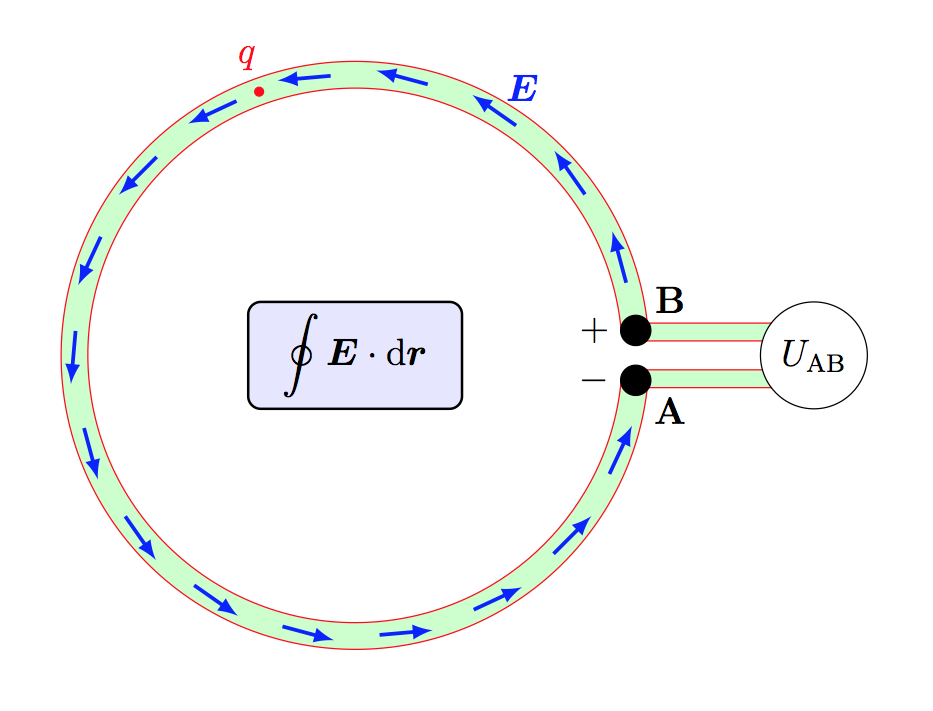
\includegraphics[width=150pt]{images/induktion}
\end{center}

Das Linienintegral des elektrischen Feldes {\"u}ber die geschlossene Schleife ist gleich der Induktionsspannung $U_{ind}$:
\begin{equation*}
	U_{ind} = \oint E\ dr = - \frac{d}{dt} \iint_A B\ dA = -\frac{d\Phi_B}{dt}
\end{equation*}


\end{multicols*}
\end{document}